
\chapter{Multiclass Classification}
\begin{definition}[Binary classification]
	Given an input $\mathscr{X}$, an unknown distribution $D$ over $\mathscr{X}\times \{-1,1\}$
	a training set D compute a function f.
\end{definition}

\begin{definition}[Multiclass classification]
	Given an input $\mathscr{X}$ and a number K of classes, an unknown distribution $D$ over $\mathscr{X}\times K$
	a training set D compute a function f.
\end{definition}

None of the current methods work.

The main idea is to modify the perceptron by adding multiple lines. There are two approaches to this.

\section{One vs All (OVA)}

For each label L define a binary problem. All examples with L are positive, the rest is negative.

This poses a problem related to some areas in which it can either be two classes or none at all.

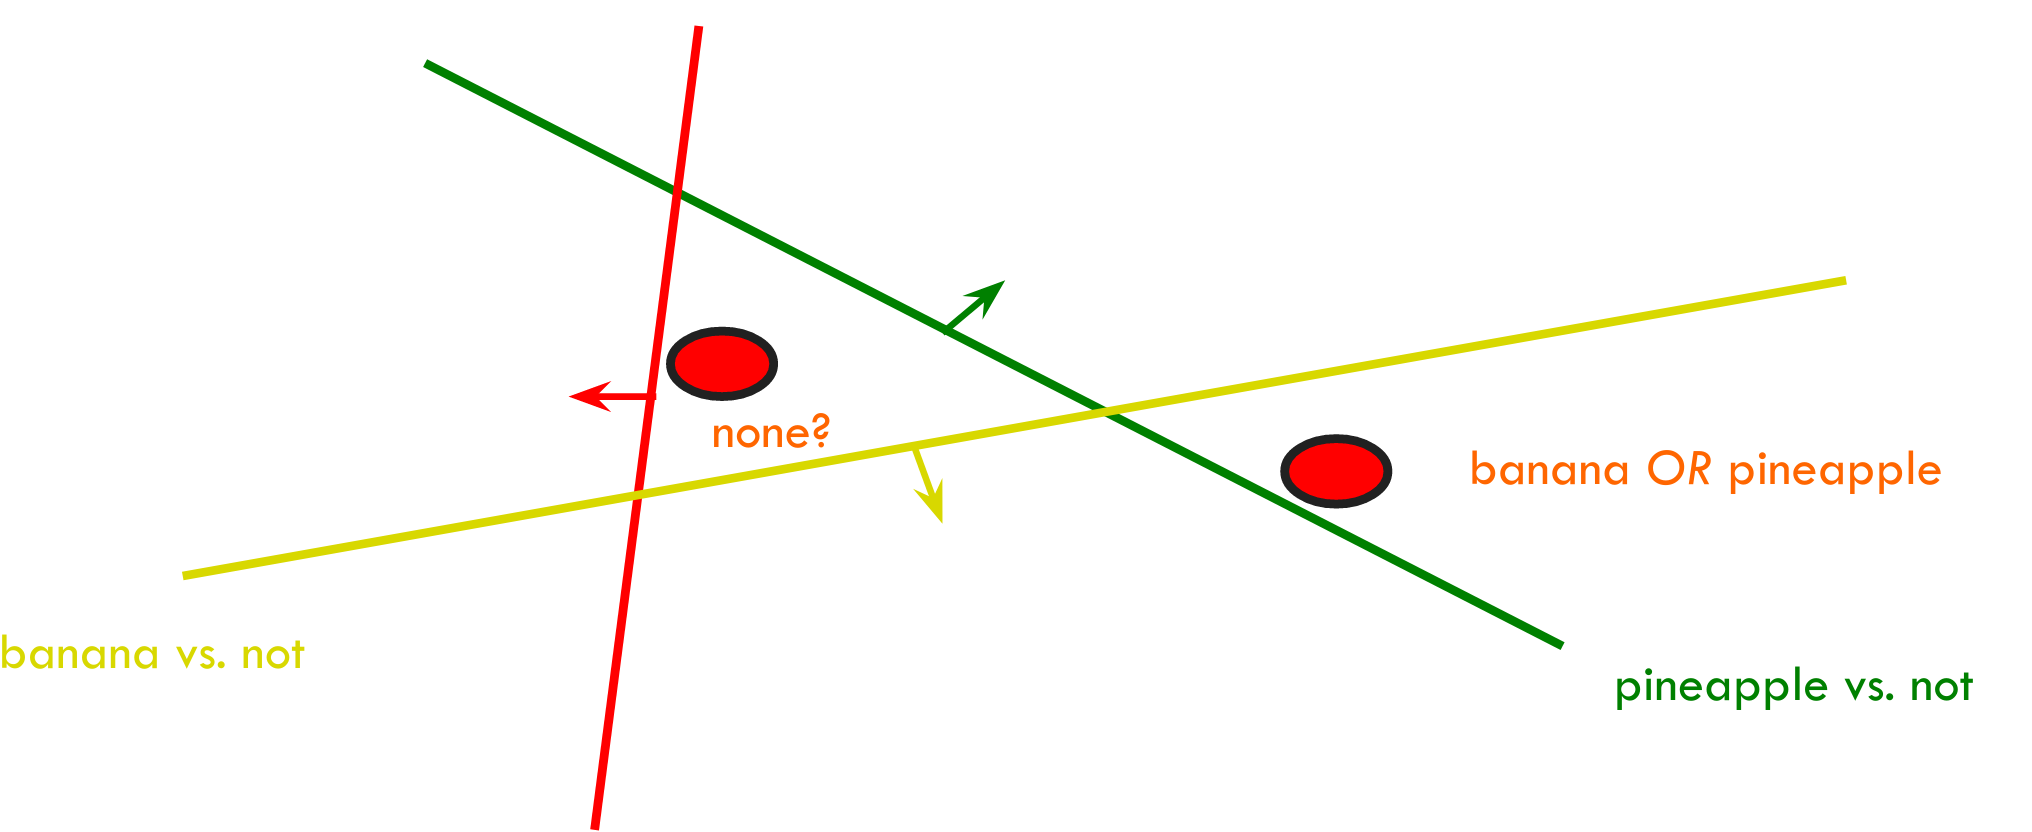
\includegraphics[scale=0.1]{multiclass}
 How to classify? 

Generally speaking the classifier should provide a level of confidence. To calculate this value we need to use decision boundaries and its distance from the hyperplane.
 
\section{All vs All (AVA)}
The idea behind AVA is to pair up each permutation of 1v1 pairs. Then, the classifier will receives all examples of i as a +1 and -1 for the j class. When a test point arrives we evaluate on all the $F_{ij}$ classifiers. 

\section{Summary}
AVA has faster training time but a slower test time. AVA has more chances of error at test time.

\textbf{Evaluation} comes when we need to evaluate a specific performance of an algorithm. Can be done through microaveraging, average over the examples, or macroaveraging, average of the average of each label.

